% =============================================================================
% Chapter 12: Text Generation
% =============================================================================
\chapter{Text Generation}
\label{ch:text-generation}

\begin{objectives}
    \item Understand autoregressive generation
    \item Master temperature scaling
    \item Implement top-k and top-p (nucleus) sampling
    \item Use repetition penalty
    \item Build an interactive generation interface
\end{objectives}

% -----------------------------------------------------------------------------
\section{Autoregressive Generation}
% -----------------------------------------------------------------------------

Generation works by repeatedly predicting the next token:

\begin{algorithm}[H]
\caption{Autoregressive Text Generation}
\begin{algorithmic}[1]
\Require Prompt tokens, model, max tokens
\State tokens $\gets$ encode(prompt)
\While{len(tokens) $<$ max\_length \textbf{and} tokens[-1] $\neq$ EOS}
    \State logits $\gets$ model(tokens)[-1]  \Comment{Last position logits}
    \State next\_token $\gets$ sample(logits)  \Comment{Sampling strategy}
    \State tokens.append(next\_token)
\EndWhile
\State \Return decode(tokens)
\end{algorithmic}
\end{algorithm}

\begin{lstlisting}[style=python, caption={Core generation loop from generate.py}]
@torch.no_grad()
def generate(
    model: GPT,
    tokenizer: TryLMTokenizer,
    prompt: str,
    max_new_tokens: int = 100,
    temperature: float = 1.0,
    top_k: int = 0,
    top_p: float = 1.0,
) -> str:
    model.eval()
    input_ids = torch.tensor([tokenizer.encode(prompt)])

    for _ in range(max_new_tokens):
        # Get logits for last position
        outputs = model(input_ids)
        next_token_logits = outputs["logits"][0, -1, :]

        # Apply sampling
        next_token_logits = next_token_logits / temperature
        if top_k > 0:
            next_token_logits = top_k_filtering(next_token_logits, top_k)
        if top_p < 1.0:
            next_token_logits = top_p_filtering(next_token_logits, top_p)

        # Sample
        probs = F.softmax(next_token_logits, dim=-1)
        next_token = torch.multinomial(probs, num_samples=1)

        # Append and check for EOS
        input_ids = torch.cat([input_ids, next_token.unsqueeze(0)], dim=1)
        if next_token.item() == tokenizer.eos_id:
            break

    return tokenizer.decode(input_ids[0].tolist())
\end{lstlisting}

% -----------------------------------------------------------------------------
\section{Temperature}
% -----------------------------------------------------------------------------

\textbf{Temperature} controls randomness by scaling logits before softmax:

\begin{equation}
p_i = \frac{\exp(z_i / T)}{\sum_j \exp(z_j / T)}
\end{equation}

\begin{itemize}
    \item $T < 1$: Sharper distribution (more deterministic)
    \item $T = 1$: Original distribution
    \item $T > 1$: Flatter distribution (more random)
\end{itemize}

\begin{figure}[H]
\centering
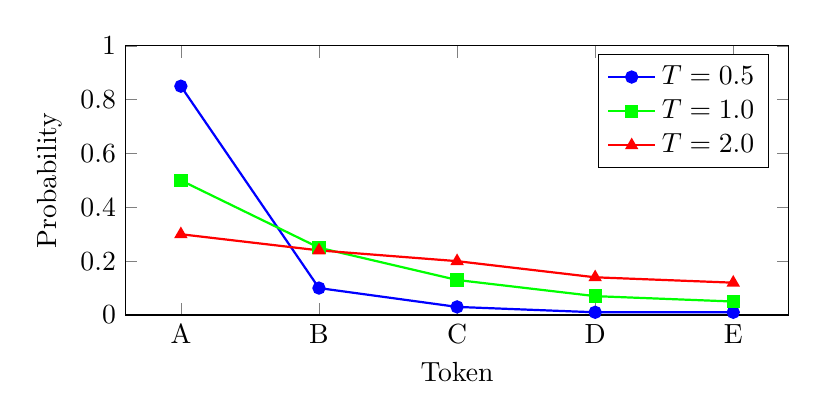
\begin{tikzpicture}
    \begin{axis}[
        width=10cm,
        height=5cm,
        xlabel={Token},
        ylabel={Probability},
        ymin=0, ymax=1,
        legend pos=north east,
        xtick={1,2,3,4,5},
        xticklabels={A, B, C, D, E},
    ]
        % T=0.5
        \addplot[thick, blue, mark=*] coordinates {
            (1, 0.85) (2, 0.10) (3, 0.03) (4, 0.01) (5, 0.01)
        };
        \addlegendentry{$T=0.5$}

        % T=1.0
        \addplot[thick, green, mark=square*] coordinates {
            (1, 0.50) (2, 0.25) (3, 0.13) (4, 0.07) (5, 0.05)
        };
        \addlegendentry{$T=1.0$}

        % T=2.0
        \addplot[thick, red, mark=triangle*] coordinates {
            (1, 0.30) (2, 0.24) (3, 0.20) (4, 0.14) (5, 0.12)
        };
        \addlegendentry{$T=2.0$}
    \end{axis}
\end{tikzpicture}
\caption{Effect of temperature on probability distribution}
\label{fig:temperature}
\end{figure}

% -----------------------------------------------------------------------------
\section{Top-k Filtering}
% -----------------------------------------------------------------------------

\textbf{Top-k sampling} keeps only the $k$ most likely tokens:

\begin{lstlisting}[style=python, caption={Top-k filtering from generate.py}]
def top_k_filtering(logits: Tensor, k: int) -> Tensor:
    if k <= 0:
        return logits

    # Find the k-th largest value
    values, _ = torch.topk(logits, k)
    min_value = values[-1]

    # Set all values below threshold to -inf
    return torch.where(
        logits < min_value,
        torch.full_like(logits, float("-inf")),
        logits,
    )
\end{lstlisting}

% -----------------------------------------------------------------------------
\section{Top-p (Nucleus) Sampling}
% -----------------------------------------------------------------------------

\textbf{Top-p sampling} keeps the smallest set of tokens whose cumulative probability exceeds $p$:

\begin{lstlisting}[style=python, caption={Top-p filtering from generate.py}]
def top_p_filtering(logits: Tensor, p: float) -> Tensor:
    sorted_logits, sorted_indices = torch.sort(logits, descending=True)
    cumulative_probs = torch.cumsum(F.softmax(sorted_logits, dim=-1), dim=-1)

    # Find cutoff index
    sorted_indices_to_remove = cumulative_probs > p
    sorted_indices_to_remove[1:] = sorted_indices_to_remove[:-1].clone()
    sorted_indices_to_remove[0] = False

    # Remove tokens beyond cutoff
    indices_to_remove = sorted_indices[sorted_indices_to_remove]
    logits[indices_to_remove] = float("-inf")

    return logits
\end{lstlisting}

\begin{keypoint}
Top-p is more adaptive than top-k:
\begin{itemize}
    \item When the model is confident, fewer tokens are kept
    \item When uncertain, more tokens are allowed
\end{itemize}
\end{keypoint}

% -----------------------------------------------------------------------------
\section{Repetition Penalty}
% -----------------------------------------------------------------------------

To avoid repetitive text, penalize tokens that have already appeared:

\begin{lstlisting}[style=python]
def apply_repetition_penalty(
    logits: Tensor,
    generated_tokens: list[int],
    penalty: float = 1.2,
) -> Tensor:
    for token_id in set(generated_tokens):
        if logits[token_id] > 0:
            logits[token_id] /= penalty
        else:
            logits[token_id] *= penalty
    return logits
\end{lstlisting}

% -----------------------------------------------------------------------------
\section{Generation Examples}
% -----------------------------------------------------------------------------

\begin{lstlisting}[style=shell]
# Basic generation
uv run trylm generate "Once upon a time"

# Adjust parameters
uv run trylm generate "The princess" \
    --temperature 0.8 \
    --top-k 50 \
    --top-p 0.9 \
    --max-tokens 200

# Interactive mode
uv run trylm generate -i
\end{lstlisting}

\subsection{Interactive Mode}

\begin{lstlisting}[style=shell, numbers=none]
TryLM Interactive Mode
Commands: :temp <v>, :top_p <v>, :max <v>, :quit

> Once upon a time there was a little rabbit.
The rabbit liked to hop in the garden. One day,
the rabbit found a big carrot...

> :temp 0.5
Temperature set to 0.5

> The king
The king was very happy. He had a beautiful castle.
\end{lstlisting}

% -----------------------------------------------------------------------------
\section{Summary}
% -----------------------------------------------------------------------------

\begin{summary}
    \item \textbf{Autoregressive generation}: predict one token at a time, append, repeat
    \item \textbf{Temperature}: controls randomness ($<1$ = focused, $>1$ = diverse)
    \item \textbf{Top-k}: keep only $k$ most likely tokens
    \item \textbf{Top-p (nucleus)}: keep tokens until cumulative probability $> p$
    \item \textbf{Repetition penalty}: discourage repeating tokens
    \item Recommended defaults: temperature=0.8, top\_p=0.9, top\_k=50
\end{summary}
